\documentclass{article}


\usepackage[utf8]{inputenc}
\usepackage[T1]{fontenc}
\usepackage[a4paper,includeheadfoot,margin=2.54cm,includehead]{geometry}
\usepackage[skip=2mm, indent=5mm]{parskip}
\usepackage[sfdefault]{notomath}
\usepackage{float}
\usepackage{graphicx}
\usepackage[figurename=Fig.]{caption}
\usepackage[unicode,bookmarks,colorlinks,breaklinks]{hyperref}  
\usepackage{color}
\usepackage{fancyhdr}


\begin{document}

% ------------------------------------------------
% | % Título, autor, materia, fecha, ciudad... % |
% ------------------------------------------------
\newcommand{\titulo}{Documentación del proyecto Boxing Game}
\newcommand{\escuela}{Escuela de Ingeniería Informática}
\newcommand{\autorAngel}{Ángel Iglesias Préstamo}
\newcommand{\autorDiego}{Diego Martín Fernández}
\newcommand{\asignatura}{Informática Audiovisual}
\newcommand{\universidad}{Universidad de Oviedo}
\newcommand{\fecha}{\today} % Muestra por defecto la fecha actual

% ----------------------------------------------------------
% | % Establecemos un estilo para el encabezado y el pie % |
% ----------------------------------------------------------
\pagestyle{fancy}
\fancyhf{}

\renewcommand{\headrulewidth}{0.5pt}
\renewcommand{\footrulewidth}{0.5pt}

\fancyhead[RO]{\nouppercase{\titulo\hfill\asignatura}}
\fancyfoot[CE,CO]{\thepage}

% --------------------------------------------------------------------
% | % Establecemos el estilo de los enlaces y referencias-cruzadas % |
% --------------------------------------------------------------------

\definecolor{blueUniovi}{RGB}{0,51,170}
\hypersetup{
    linkcolor=blueUniovi,
    citecolor=blueUniovi,
    filecolor=black,
    urlcolor=blueUniovi,
    bookmarksnumbered=true,
    bookmarksopen=true,
    bookmarksopenlevel=1,
    pdfpagemode=UseOutlines
}

% --------------------------------------------------------------
% | % Establecemos el estilo de algunas secciones y párrafos % |
% --------------------------------------------------------------

\makeatletter
\renewcommand\paragraph{\@startsection{paragraph}{4}{\z@}%
    {3.25ex \@plus1ex \@minus.2ex}%
    {0pt}%
    {\normalfont\normalsize\bfseries}}
\makeatother

% -----------------------------
% | % Portada del documento % |
% -----------------------------
\newcommand{\HRule}{\rule{\linewidth}{0.5mm}}
\begin{titlepage}
    \centering
    
\includegraphics[width=0.3\textwidth]{img/uniovi.eps}
    \vfill
    \HRule
    \vspace{0.4cm}
    {\huge\bfseries\titulo\par}
    \vspace{1.5cm}
    {\Large\itshape\autorAngel\par\vspace{0.1cm}\autorDiego\par}
    \vspace{0.4cm}
    \HRule
    \vspace{1.5cm}
    {\LARGE\escuela\par}
    \vspace{0.5cm}
    {\Large\asignatura\par}
    \vfill
    {\large\universidad\par}
    \fecha
    \vfill
\end{titlepage}

% -----------------------------------------
% | % Tabla de contenidos del documento % |
% -----------------------------------------
\renewcommand{\contentsname}{Tabla de contenidos}
\tableofcontents{}
\newpage

% ---------------------------------------
% | % Empezamos el documento en sí :D % |
% ---------------------------------------

\section{Introducción}

\href{https://angelip2303.github.io/boxing-docs/}{Boxing Game} es el proyecto en equipo de la asignatura de Informática Audiovisual desarrollado por Ángel Iglesias Préstamo y Diego Martín Fernández. Se trata de un mini-juego de boxeo controlado mediante una cámara. La presente es la documentación del mismo. En esta se desarrolla el proceso seguido para diseñar el sistema en el apartado \ref{section:design}. En la sección \ref{section:development} se describe el proceso seguido para la correcta implementación del mini-juego planteado en el punto anterior: esto es, un breve comentario acerca de las tecnologías utilizadas. Posteriormente, en el apartado \ref{section:manual} se redactan una serie de consideraciones a tener en cuenta para poder interactuar correctamente con el sistema. Finalmente, en la sección \ref{section:work}, se justifica el trabajo aportado por cada uno de los miembros del equipo.

\section{Diseño}
\label{section:design}

\begin{figure}[h]
    \centering
    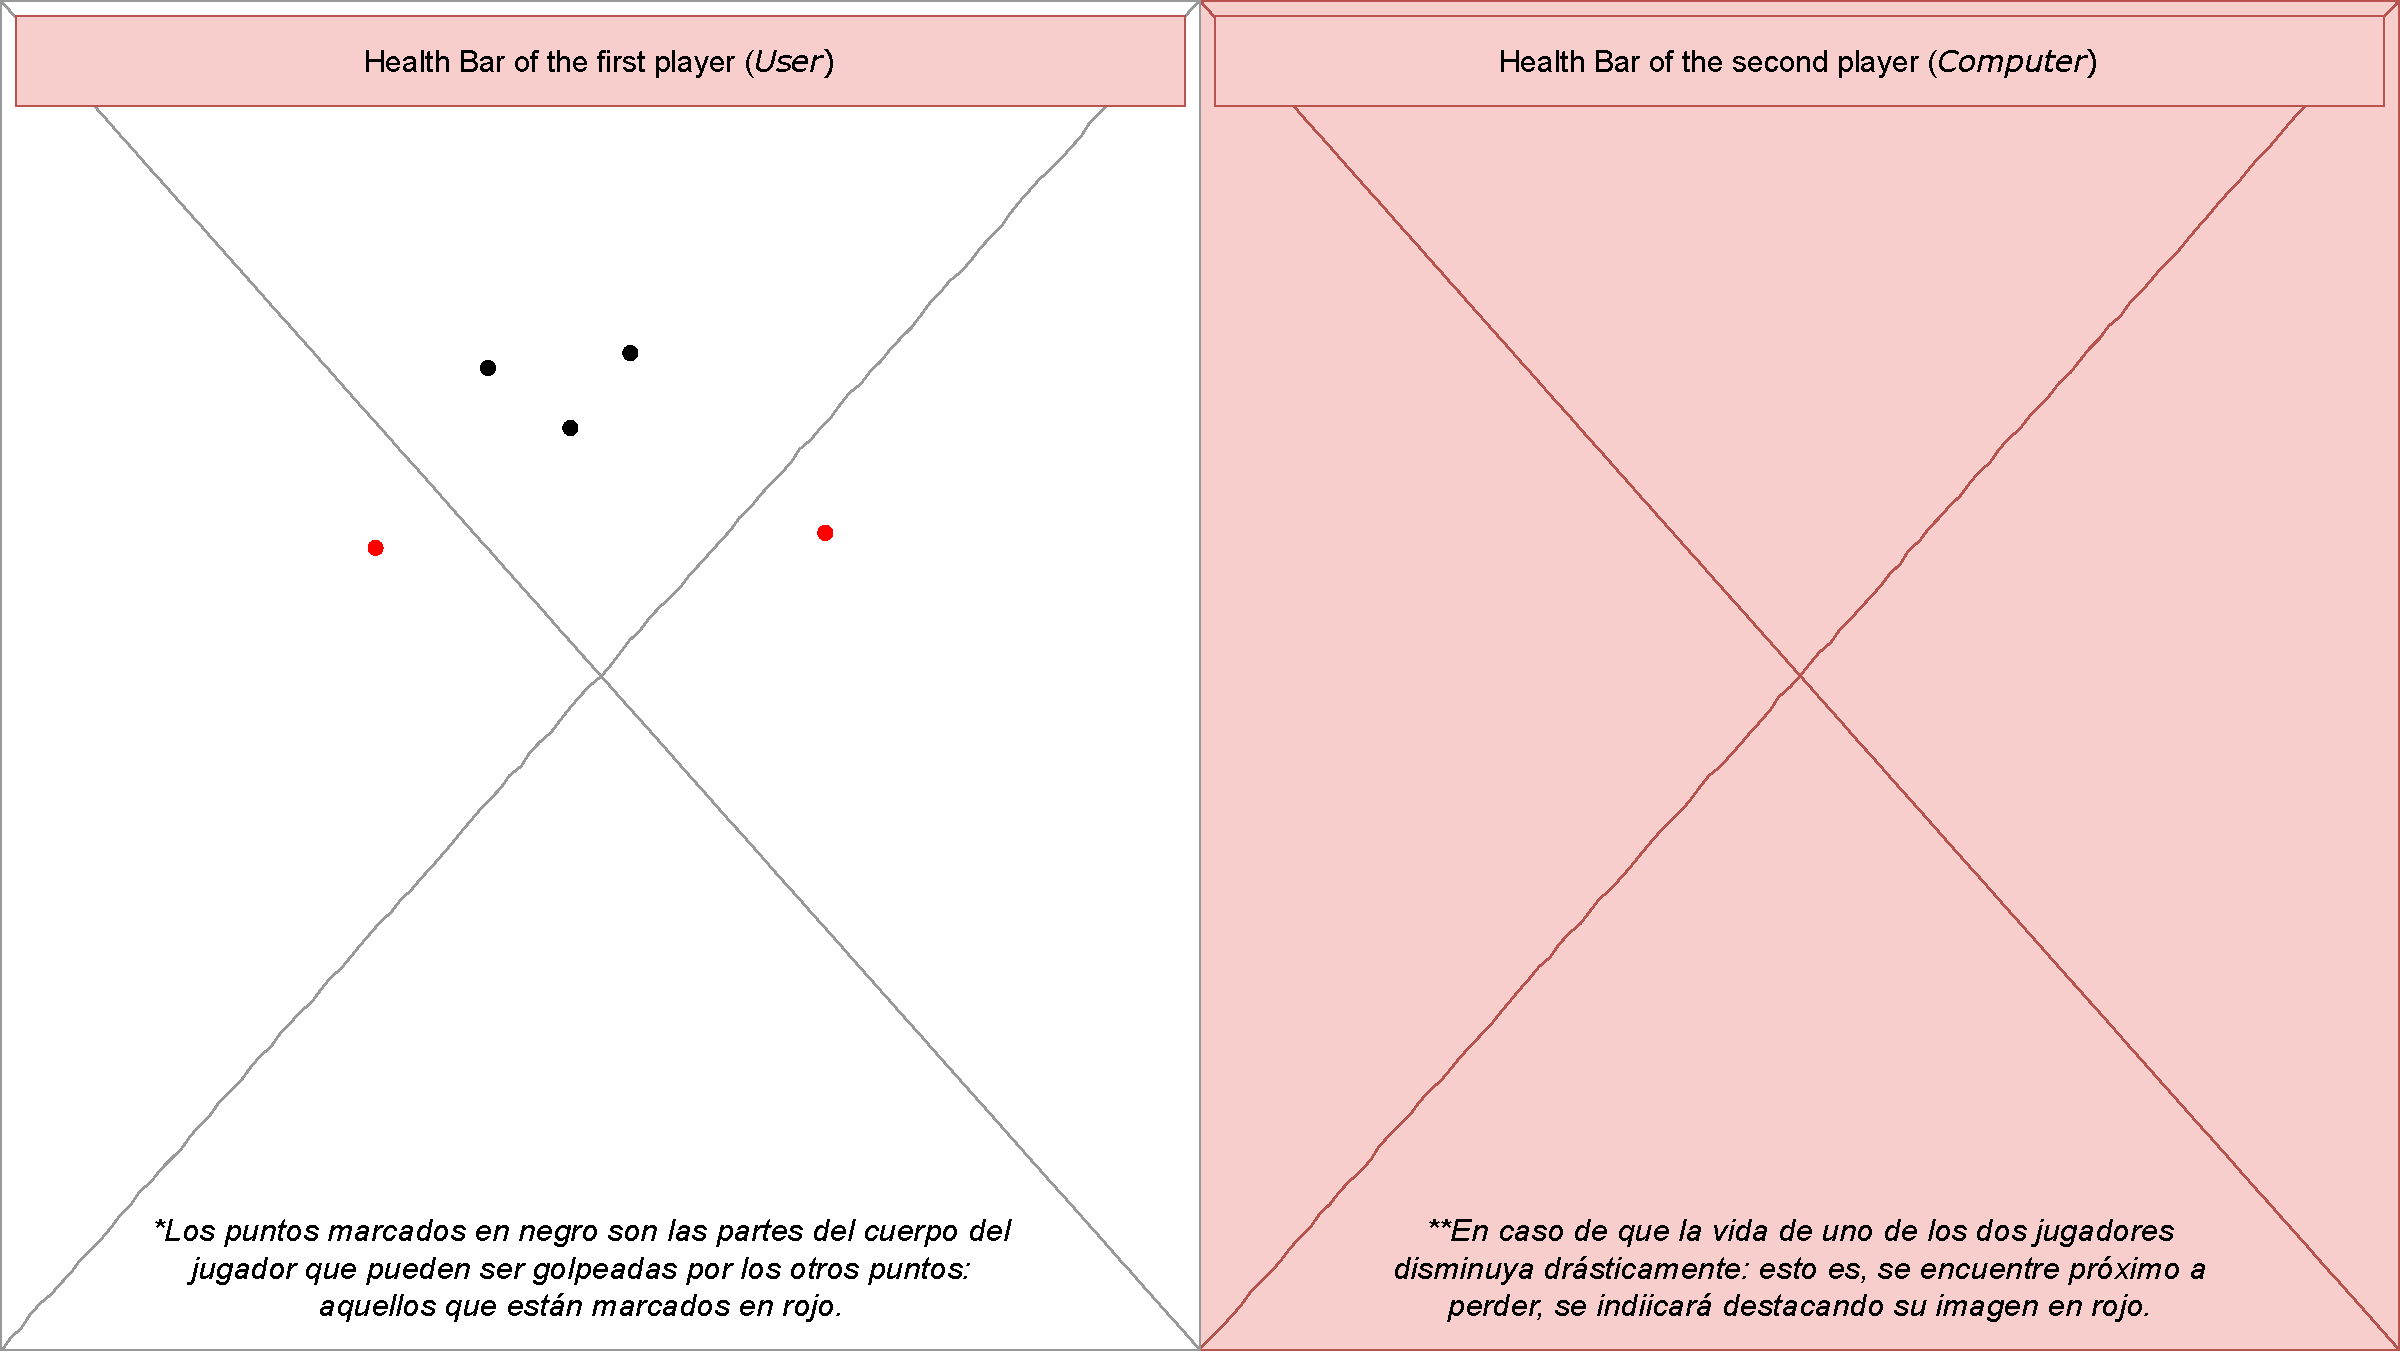
\includegraphics[width=\textwidth]{img/wireframe1}
    \caption{Wireframe de la pantalla principal de la interfaz de usuario}
    \label{fig:mesh1}
\end{figure}

\subsection{Colores}

\subsection{Tipografía}

\section{Desarrollo}
\label{section:development}

\subsection{Tecnologías utilizadas}

\subsubsection{p5.js}

\href{https://p5js.org/es/}{p5.js} es la biblioteca de JavaScript que hemos utilizado en la asignatura para desarrollar proyectos de programación creativa. En nuestro caso, nos ha permitido implementar un sistema audiovisual donde el usuario interactúa mediante una cámara conectada a su dispositivo. Podríamos resumir el uso que le damos a \textit{p5.js} como el marco de trabajo para permitir la interacción cliente-sistema y viceversa. No sólo se puede controlar al jugador, sino que también se recibe información sobre el estado de la partida: una barra de vida, colores que nos destacan las partes del cuerpo que golpean y las que pueden ser golpeadas; más de eso en la sección \ref{section:design}.

\subsubsection{ml5.js}

\href{https://ml5js.org/}{ml5.js} es una biblioteca de JavaScript que permite el desarrollo de aplicaciones que exploren el uso de inteligencia artificial en el navegador. La mayor ventaja, en nuestro caso, que presenta es que permite una integración muy sencilla con \textit{p5.js}. De esta forma, permite el uso del modelo \texttt{ImageNet} para la detección de \textit{Poses}: esto es, nos facilita la detección de las partes del cuerpo de sendos jugadores.

De alguna forma podríamos decir que el \textit{stack} formado por las dos tecnologías mencionadas es realmente el núcleo del proyecto.

\section{Manual}
\label{section:manual}

\subsection{Requisitos}

\paragraph{Activar la aceleración por Hardware} \mbox{} -- Para alcanzar el mayor rendimiento de la aplicación se recomienda activar la aceleración por Hardware. Esto permite al sistema el uso de la GPU para que esta se encargue de ejecutar el modelo de aprendizaje automático \texttt{ImageNet} para la detección de \textit{Poses}. Se deben seguir los siguientes pasos:

\begin{enumerate}
    \item Acceda a la configuración de su navegador.
    \item Busque \textit{Aceleración por Hardware} y active esa funcionalidad.
\end{enumerate}

\paragraph{Permitir el uso de la cámara} \mbox{} -- La forma en la que se interactúa con el sistema es a través de la cámara. Es por eso que se deberá permitir el uso de la misma para poder jugar a \textit{Boxing Game}.

\subsection{Uso}

\section{Reparto del trabajo}
\label{section:work}

\end{document}
